\documentclass[pdftex,12pt]{article}

\usepackage[utf8]{inputenc}
\usepackage[english]{babel}
\usepackage[english]{isodate}
\usepackage[parfill]{parskip}
\usepackage[pdftex]{graphicx}
\usepackage{todonotes} % \todo{note} \listoftodos
\usepackage{microtype}
\usepackage{titling}
\usepackage{booktabs}
\usepackage{multirow}
\usepackage{hyperref}
\usepackage{float}
\usepackage{longtable}
\usepackage{tablefootnote}
\usepackage{chngpage}
\usepackage{caption}
\usepackage{colortbl}
\usepackage[margin=1in,top=0.5in]{geometry}

% Commands
\newcommand{\HRule}{\rule{\linewidth}{0.5mm}}

\title{Maxwell Katz for Dummies}
\author{Harrison Katz}
\date{\today}

\begin{document}
\pagenumbering{Roman}

% Title Page
\begin{titlepage}
    \begin{center}
        \ % starts a paragraph so tex is happy
        \textsc{\huge \thetitle}\\
        \textsc{An Instruction Manual}\\[1em]
        \HRule \\[1em]

        \begin{figure}[h!]
            \centering
            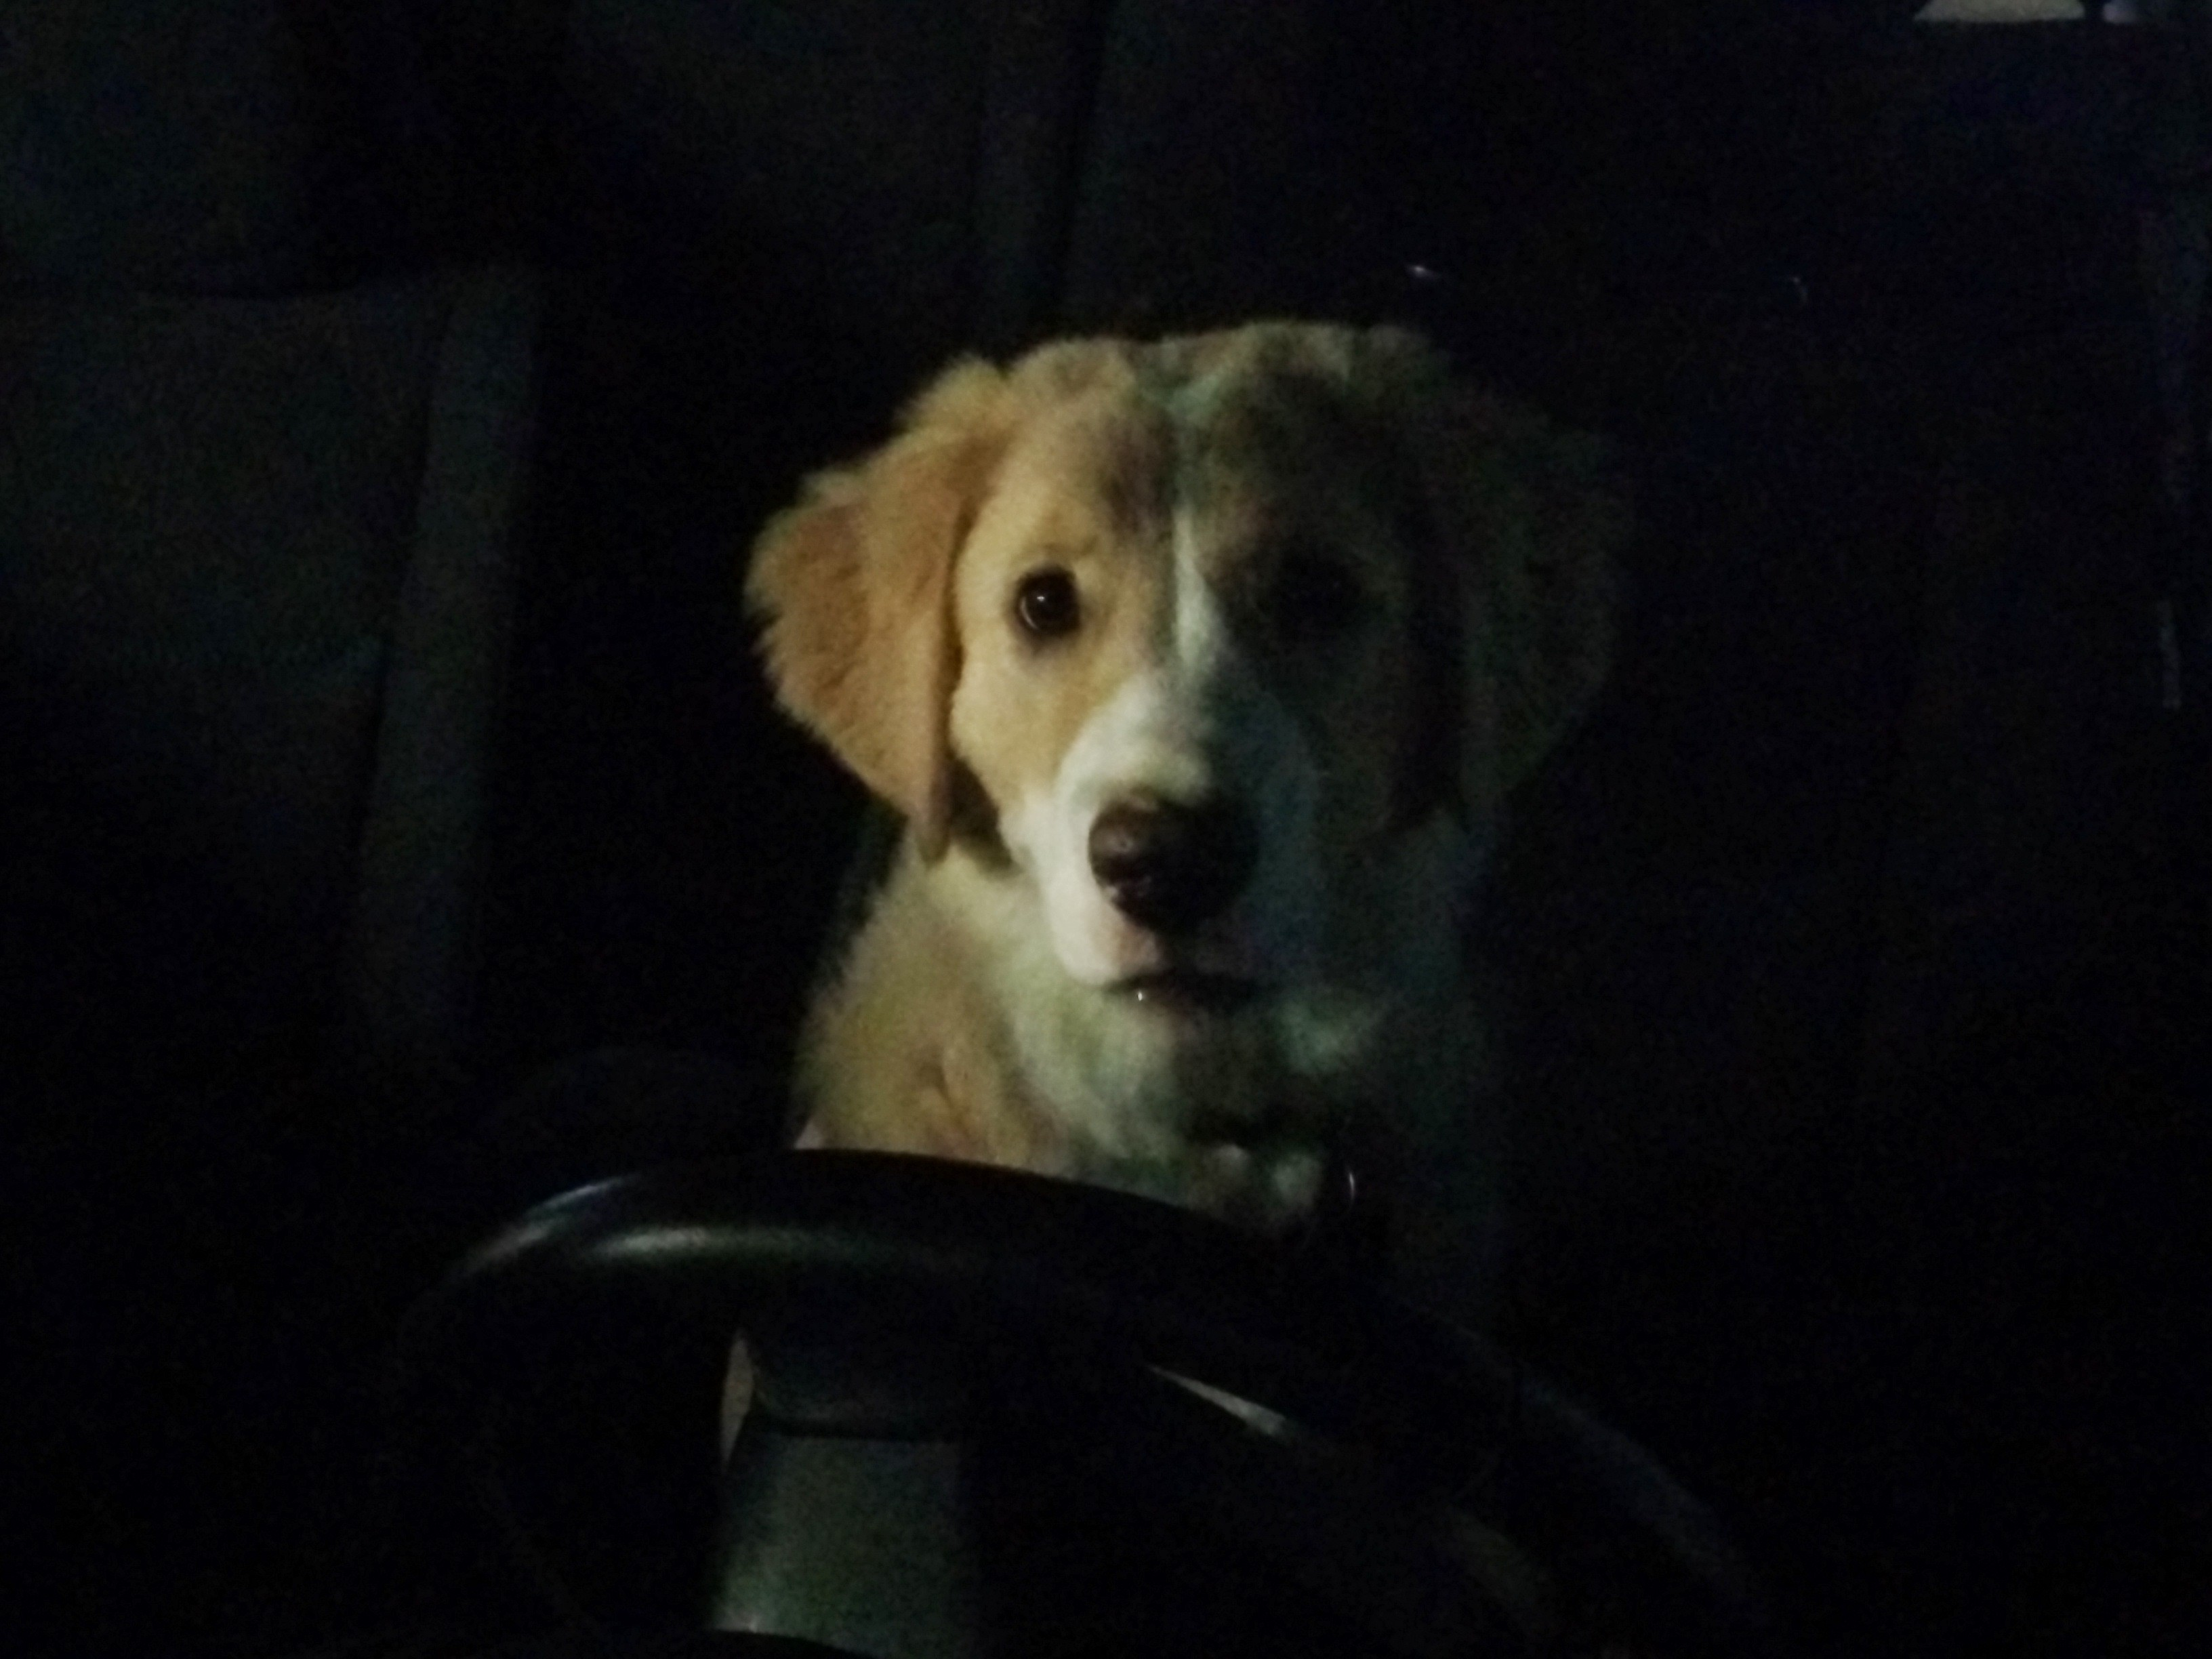
\includegraphics[width=.75\textwidth]{./images/max/title.jpg}
            \caption{Maxwell learning to operate a motor-vehicle.}
            \label{fig:max_title}
        \end{figure}

        % Bottom of the page
        \vfill
        {
            \large \theauthor \  --- \large \thedate
        }

    \end{center}
\end{titlepage}


% Contents
\newpage
\tableofcontents

% % Figures
% \newpage
% \listoffigures

% Document
\newpage
\pagenumbering{arabic}

\section{Introduction}

So, you've been wrangled into babysitting a Maxwell.
\emph{Sigh.}
What are you going to do?
Max is a rambunctious, destructive, incorrigible goofball,
yet he will tug at your heartstrings with his lovable face and ears.
What should you do?
What does he eat?
What does he do for fun?
What happens in the case of an emergency?!
All of this and more will be answered in the manual.

\bigskip

\begin{figure}[h!]\label{fig:walking_himself}
    \centering
    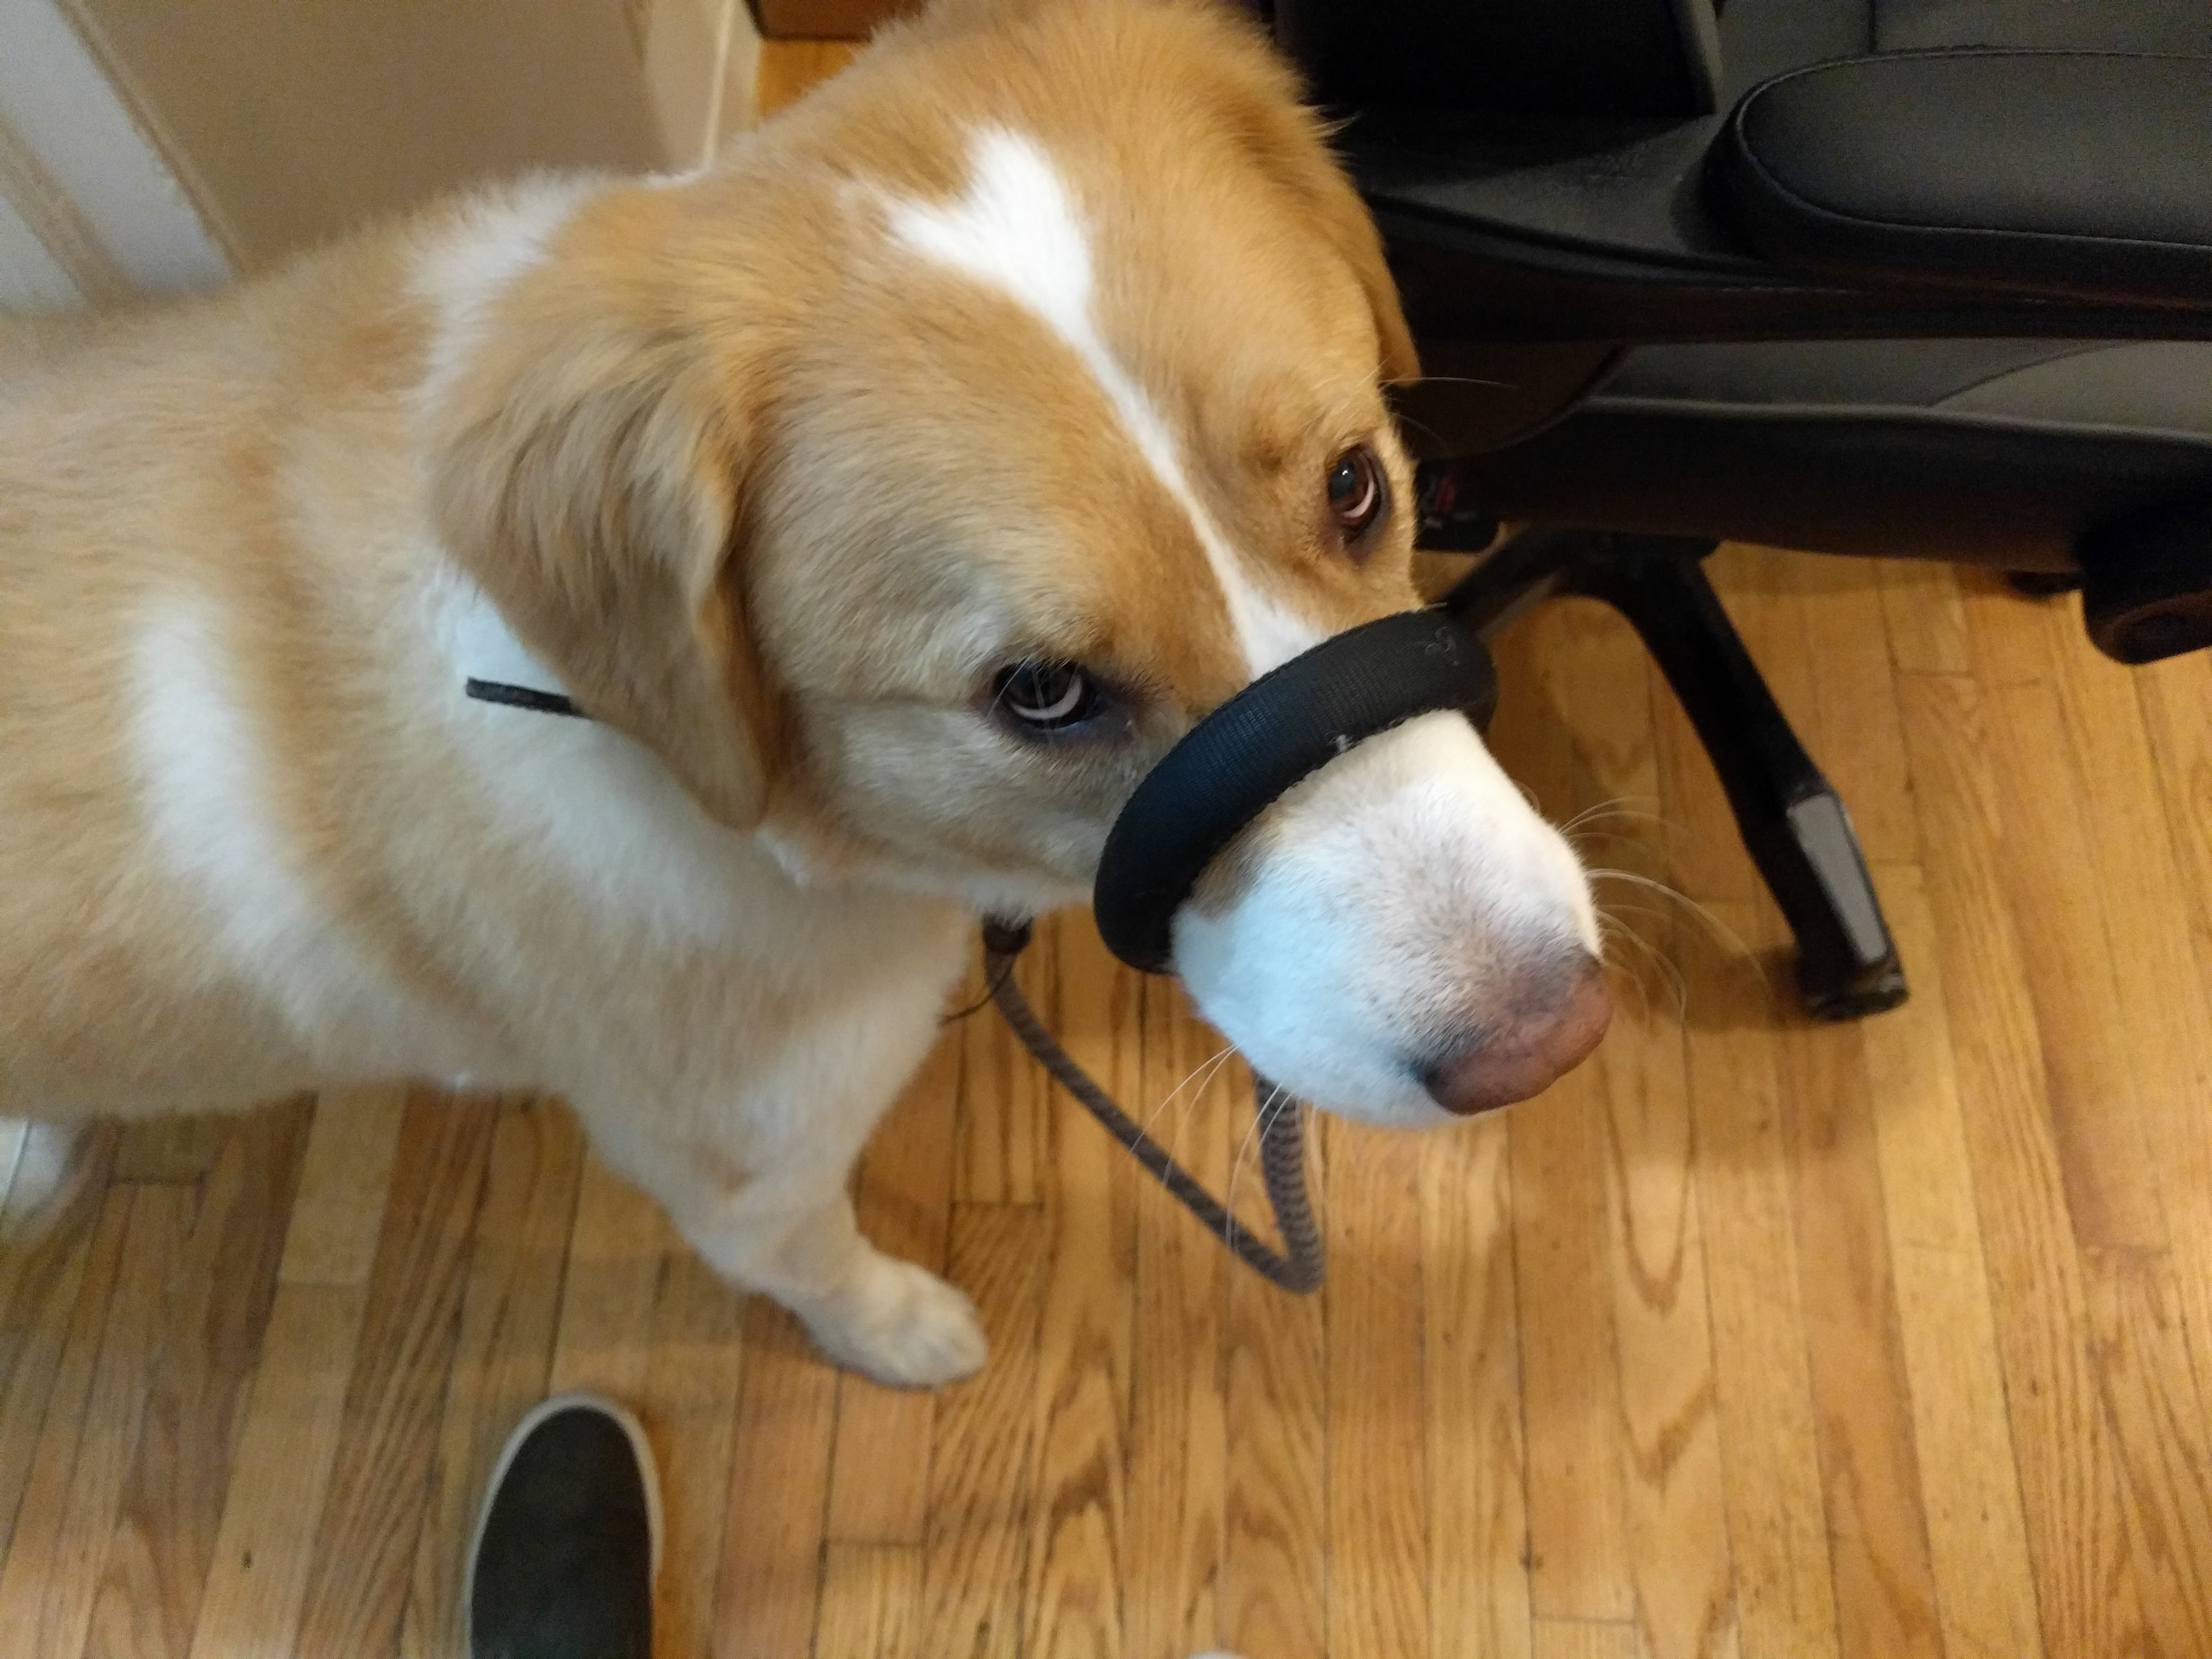
\includegraphics[width=.75\textwidth]{./images/max/walking_himself.jpg}
    \caption*{``Max doesn't like to walk himself\ldots''}
\end{figure}

\newpage
\section{Emergency Information}

\begin{table}[H]
    \begin{longtable}{@{}ll@{}}
        \toprule
        \multicolumn{2}{c}{Pet Information}                                                                                    \\ \midrule
        Name          & Maxwell Katz                                                                                           \\
        Answers to    & ``Max!'' ``Maxwell'' ``*whistle* Come here!''                                                                \\
        Breed         & Golden Retriever / Great Pyrenees                                                                      \\
        Color         & Golden White (Toasted Marshmallow)                                                                    \\
        Weight        & 104 lbs                                                                                                \\
        Date of Birth & January 9th, 2014                                                                                      \\
        Health Issues & N/A                                                                                                    \\
        Allergies     & Chocolate                                                                                              \\
        Records       & Contact Harrison for an email copy of records.                                                         \\
        Other         & Has 3 extra toes, a trait of Pyrenees                                                                  \\ \midrule
        \multicolumn{2}{c}{Owner Information}                                                                                  \\ \midrule
        Name          & Harrison John Katz                                                                                     \\
        Phone \#      & 706.801.5289                                                                                           \\
        Email         & hjkatz03@gmail.com                                                                                     \\ \midrule
        \multicolumn{2}{c}{Emergency Contact}                                                                                  \\ \midrule
        Name          & Laura Katz                                                                                             \\
        Relation      & Mother of Harrison Katz                                                                                \\
        Phone \#      & 706.612.4572                                                                                           \\
        Email         & ldkatz38@gmail.com                                                                                     \\ \midrule
        \multicolumn{2}{c}{Veterinary Information (temporary)}                                                                             \\ \midrule
        Name          & Washington Square Animal Hospital                                                                      \\
        Phone \#      & 212.674.1670                                                                                           \\
        Address       & \multirow{3}{*}{\begin{tabular}[c]{@{}l@{}}23 E 9th St.\\ NY, NY\\ 10003\end{tabular}} \\
                      &                                                                                                        \\
                      &                                                                                                        \\
        Website       & \url{http://washingtonsquarevet.com}                                                                      \\
        %Email         & info@peachtreehillsvet.com                                                                             \\
        Hours         & Mon-Fri, 9am-6pm; Sat 9am-3pm; Sun Closed                                                                       \\
        Emergency     & \url{http://www.washingtonsquarevet.com/Emergency\_Hospitals.html}
    \end{longtable}
    \label{tab:information}
\end{table}

\newpage
\section{Schedule}

Maxwell's schedule is extremely rigorous, and must be kept with the up most scrutiny.
He requires attention quite literally 24 hours a day, 7 days a week, and without this given to him, I fear he may become deprived, depressed, or worse\ldots dead.
Below is his main schedule for a normal week.

\subsection{Weekly Schedule}

\begin{table}[h]
    \caption*{Maxwell's rigorous daily schedule}
    \begin{longtable}{r|ll}
        & Weekday               & Weekend               \\ \hline \\
        Midnight \- 7 am & Sleeping
        \tablefootnote{See page~\pageref{fig:sleeping}}
        & Sleeping              \\
        8 am            & Morning Walk (E,O)
        \tablefootnote{Pee and Poop}
        & Morning Walk (E,O)    \\
        9 am            & Breakfast             & Breakfast             \\
        10 am           & Sleeping              & Play Time             \\
        11 am           & Sleeping              & Play Time             \\
        Noon            & Sleeping              & Afternoon Walk (E)
        \tablefootnote{Pee only}
        \\
        1 pm            & Sleeping              & Play Time             \\
        2 pm            & Sleeping              & Park Time             \\
        3 pm            & Sleeping              & Nap Time              \\
        4 pm            & Sleeping              & Nap Time              \\
        5 pm            & Evening Walk (E)      & Evening Walk (E)      \\
        6 pm            & Dinner                & Dinner                \\
        7 pm            & After Dinner Walk (O)
        \tablefootnote{Poop only}
        & After Dinner Walk (O) \\
        8 pm            & Play Time             & Play Time             \\
        9 pm            & Play Time             & Play Time             \\
        10 pm           & Night Walk (E)        & Night Walk (E)        \\
        11 pm           & Sleeping              & Sleeping              \\
    \end{longtable}
    \label{tab:schedule}
\end{table}

\pagebreak

\subsection{Schedule Description}
\begin{itemize}\label{itm:schedule}
    \item \textbf{Sleeping:} Max's sleeping schedule is pretty lax. He sleeps
        quite often, and is adorable the entire time. Keep in mind the following:
        \begin{itemize}
            \item Max can be pet while he is asleep
            \item Max sheds, so be aware of letting him on the bed or furniture
            \item Max sleeps in peculiar ways, this is OK
                (See page~\pageref{fig:sleeping})
        \end{itemize}
    \item \textbf{Walks:} Walking Max is no longer a chore! He has recently been fitted
        with a remote control device. (See page \pageref{sec:collar})
        \begin{itemize}
            \item Walks can be as short as 30 secs, or as long as 30 mins
            \item Some walks are pee, some poop, some both
                (See his schedule on page~\pageref{tab:schedule})
            \item Maxwell is trained to go to the bathroom on command
                (See his commands on page~\pageref{tab:commands})
            \item \textbf{Always walk Max using a leash.}
        \end{itemize}
    \item \textbf{Feeding:} Maxwell eats twice a day, once in the morning and
        once in the evening. He also receives water during each meal.
        \begin{itemize}
            \item Each meal consists of 1.5 cups of dog food
                (See page~\pageref{fig:food_bowl_filled})
            \item Max is trained to wait until eating
                (See page~\pageref{fig:food_container_open})
            \item Max eats fast, and he should be walked after dinner
            \item Sometimes Max doesn't eat breakfast, sometimes he doesn't eat dinner too.
                This is OK, he will eventually eat, don't fret.
        \end{itemize}
    \item \textbf{Play Time:} Max loves to play! His favorite game is tug-of-war.
        \begin{itemize}
            \item Max comes with a plethora of toys
                (See page~\pageref{itm:included_items})
            \item Max loves to play in the dirt and mud
            \item Max is very energetic; you have been warned
        \end{itemize}
\end{itemize}

\clearpage

\vspace*{\fill}

\begin{figure}[h!]
    \centering
    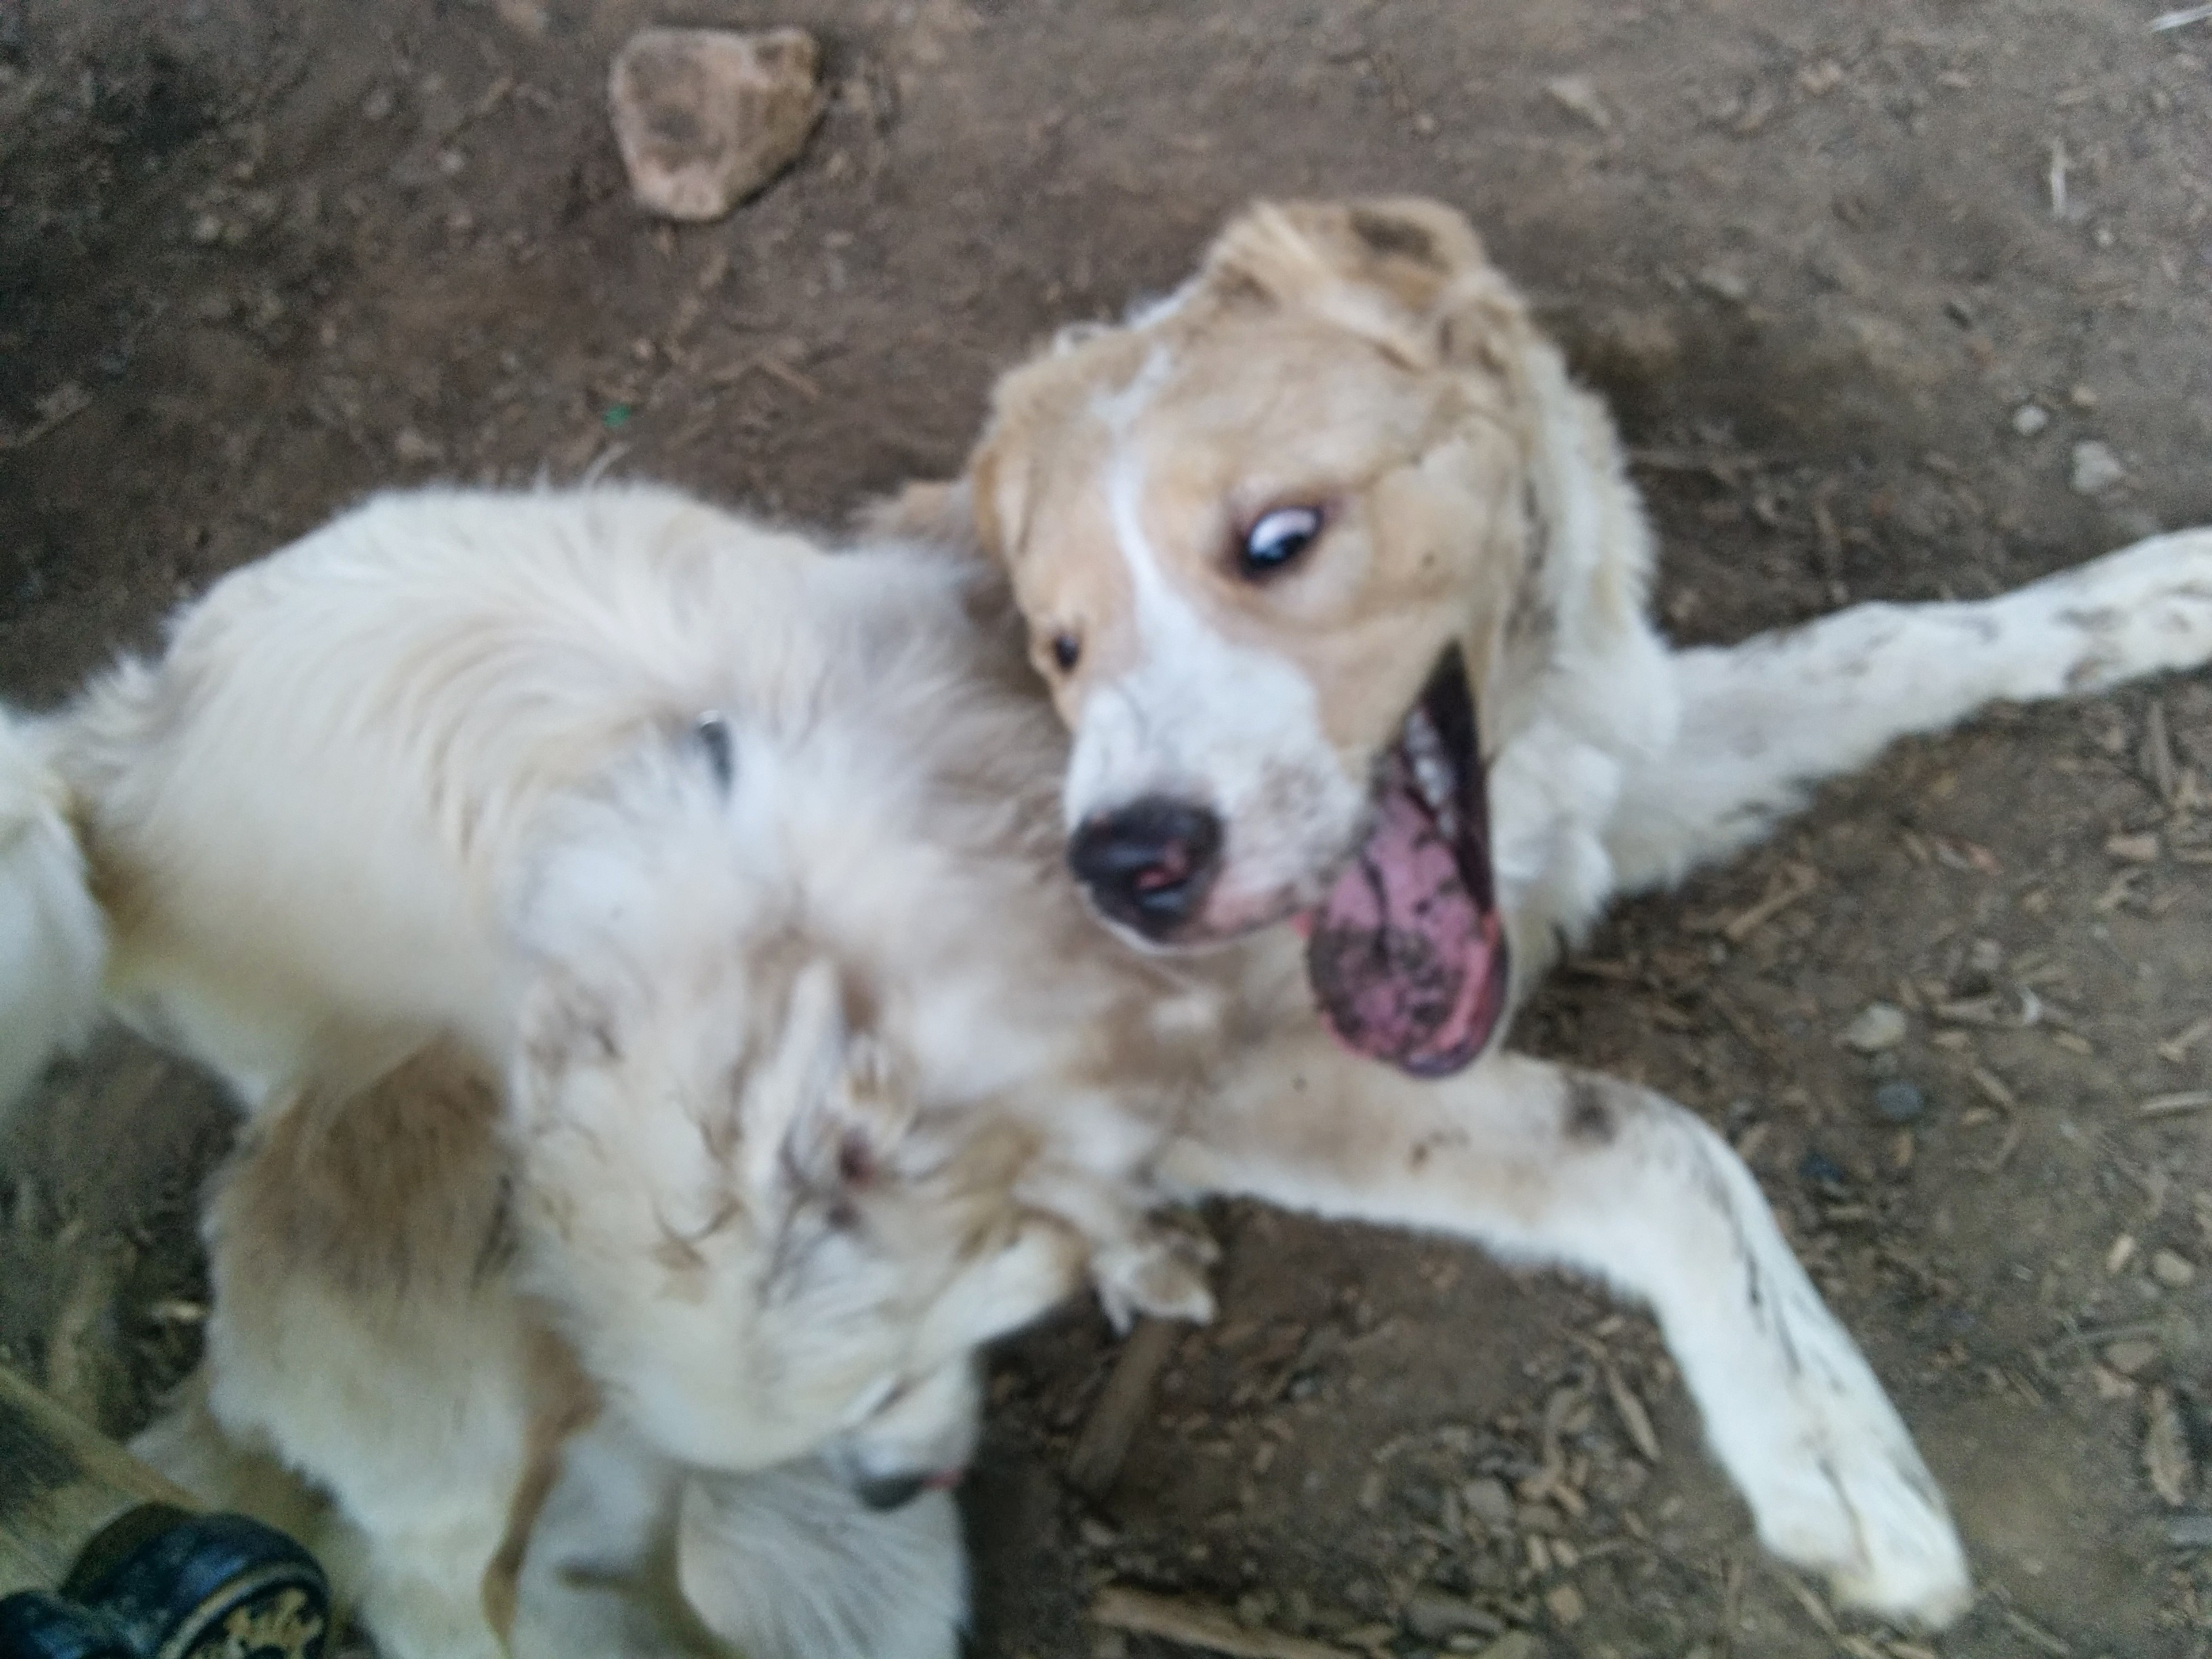
\includegraphics[width=.35\textwidth]{./images/max/at_the_park.jpg}
    \caption*{Maxwell playing at the park.}
    \label{fig:at_the_park}
\end{figure}

\bigskip

\begin{figure}[h!]\label{fig:sleeping}
    \centering
    
\includegraphics[width=.35\textwidth]{./images/max/sleeping.jpg}
    \caption*{Maxwell sleeping normally}
\end{figure}

\vspace*{\fill}

\clearpage
\newpage
\section{Included Items}

Here is a list of all of the items that you will receive for watching Maxwell.
Most of these will be in his bag.
You will not need to use all of these items, and don't worry if things get lost.
Max will probably find a toy to take home, and one to leave there.

\begin{enumerate}\label{itm:included_items}
    \item Maxwell Katz
    % \item Crate Items
    %     \begin{enumerate}
    %         \item Metal Frame
    %         \item Plastic Base
    %         \item Max's Towel
    %     \end{enumerate}
    \item Max's Cot
    \item Max's Bag
        \begin{enumerate}
            \item Treats
            \item Nail Clippers
            \item Bitter Spray
            \item Baggies
            \item Peepee Spray
            \item Good Paper Towels
            \item Furminator Brush
            \item Shampoo
            \item Toys
                \begin{enumerate}
                    \item Bone
                    \item Wubba
                    % \item Tug-of-War
                    \item Rope
                \end{enumerate}
        \end{enumerate}
    \item Food Bowls (x2)
    \item Food Container
    \item Leash
    \item Collar Bag
        \begin{enumerate}
            \item Electric Collar
            \item Remote Control
            \item Charging Kit
        \end{enumerate}
\end{enumerate}

\newpage
\section{Electric Collar}\label{sec:collar}

Max has gone through professional e-collar training to become off leash reliable.
Please make use of his e-collar throughout his stay.
You don't have to use the remote control with his commands or on walks,
but please have the collar on him at least.

\subsection{Questions about the e-collar}

\begin{itemize}
    \item Does the collar hurt Max?
        \begin{itemize}
            \item No. Even though it is an electric charge, the ``shock'' doesn't hurt.
                It's like a TENS unit that contracts the muscles around his neck.
            \item I've used it on my wrists before and it's not bad just
                a different feeling that Max understands as ``pay attention''.
        \end{itemize}
    \item How high should the remote be set to?
        \begin{itemize}
            \item It depends on how distracting of an environment Max is in.
                If it's just Max and me I usually use the 15-25 range.
                If we're at the dog park I'll use the 25-35 range.
                If Max is running off into the distance chasing a cat then I'll set it to the 70-90
                range.
            \item If Max whimpers at the shock don't worry.
                He's just being a baby.
                Make sure you \textbf{keep holding the button} until he responds, even in this case.
        \end{itemize}
    \item What should I do if Max doesn't respond to my command?
        \begin{itemize}
            \item Turn the ``volume'' up on the remote and keep calling him.
        \end{itemize}
\end{itemize}

\subsection{How to use the e-collar}
\begin{itemize}
    \item \textbf{Turning it On:}
        \begin{itemize}
            \item The \textbf{remote control} is turned on by holding
                down the black button on the back until the screen turns on.
            \item The \textbf{e-collar} has a little red dot which is magnetic. The
                remote has the same. Touch these two together and the collar
                will light up green.
        \end{itemize}
    \item \textbf{Turning it Off/Charging:}
        \begin{itemize}
            \item In general I don't turn the collar or remote off because
                they automatically turn off while charging.
            \item The charging cables plug into the back of both devices.
                Simply open up the water proof seal and plug them in.
            \item The devices will be red while charging and green when
                charged.
        \end{itemize}
    \item \textbf{Putting the Collar On:}
        \begin{itemize}
            \item Make sure that the collar and remote are both on.
            \item Put the e-collar around Max's neck in-front of his leash
                collar.
            \item Hook the e-collar at 3 holes first, then have Max look up
                and slide the e-collar back around his neck fat.
            \item Tighten the e-collar to 4 holes if it's still a bit loose.
            \item You should be able to put 2 fingers in between the collar
                and Max's neck, but it should be a tight fit.
        \end{itemize}
    \item \textbf{E-Collar Commands:}
        \begin{itemize}
            \item Some commands are special and have been associated with the e-collar stimulation.
                These commands will have you \textbf{hold down} the red stimulate button until Max performs a certain action,
                then you will release it.
            \item His command table will have instructions on e-collar use.
        \end{itemize}
\end{itemize}

\newpage
\section{Commands}

This section is all about how to speak to Max. You need to be commanding yet attentive to his mood.
Like all animals, he demands respect, and misbehaves like a child would.
He will always listen to commands better with a treat/toy in hand.
Maxwell has also been trained to listen for whistling, any command can be prefaced with a short loop-de-loop whistle to make him pay attention.
Some commands require e-collar stimulation for better performance.

\begin{table}[H]\label{tab:commands}
\begin{adjustwidth}{-4.5cm}{-4.5cm}
\begin{center}
\bgroup%
\def\arraystretch{1.3} % add padding to rows
\begin{tabular}{lp{.3\textwidth}p{.3\textwidth}p{.3\textwidth}}
\rowcolor{gray!50} Command    & Motion/E-Collar                                                  & Description                                           & Notes                                                                \\
\hline
\rowcolor{white}   Bad Dog    &                                                                  & Term of extreme discipline                            & Shouted with angry eyes                                              \\
\rowcolor{gray!25} Catch      &                                                                  & He might catch what you toss                          & Toss something to catch                                              \\
\rowcolor{white}   Come Here  & \textbf{E-collar stimulate} until he turns to come               & Get Maxwell to come to you                            & Should be prefaced with Max or whistle                               \\
\rowcolor{gray!25} Down       & Pinched fingers, downward bow motion                             & Laying down                                           & Sit, then down                                                       \\
\rowcolor{white}   Drop it    & Hold hand below mouth for item                                   & Drops item in mouth/opens mouth                       & Need to ``trade'' another item for what he has                       \\
\rowcolor{gray!25} Eh!/Uh-uh  &                                                                  & General purpose use, stop what Max is currently doing &                                                                      \\
\rowcolor{white}   Go         & Herding motion with both hands                                   & Move out of my way, go somewhere                      & Use for getting him into his crate                                   \\
\rowcolor{gray!25} Good Boy   & Petting, Smiling                                                 & Term of praise                                        &                                                                      \\
\rowcolor{white}   Go Outside &                                                                  & Get Maxwell excited, go to the door                   & Ask as a question                                                    \\
\rowcolor{gray!25} Heel       & E-collar stimulate until he's by your left side                  & Have Maxwell walk by your side                        & Keep stimulating until he's on your left side in his box. Be strict. \\
\rowcolor{white}   Leave it   & Yank leash                                                       & Leave it alone, ignore it                             & Start with Eh/Uh-uh                                                  \\
\rowcolor{gray!25} Maxwell    &                                                                  & Get his attention                                     &                                                                      \\
\rowcolor{white}   No         &                                                                  & More extreme Eh/Uh-uh                                 &                                                                      \\
\rowcolor{gray!25} Okay       &                                                                  & Release command                                       & Use to release from wait, sit, down, feeding, etc\ldots              \\
\rowcolor{white}   Place      & E-collar stimulate until all paws are on the object              & Put Max somewhere to stay                             & Place again if he gets off without a release or come when called     \\
\rowcolor{gray!25} Poopy      &                                                                  & Go poop                                               & For use outside                                                      \\
\rowcolor{white}   Potty      &                                                                  & Go pee                                                & For use outside                                                      \\
\rowcolor{gray!25} Sit        & E-collar stimulate tap, or pinched fingers, upward \break motion & Sitting                                               &                                                                      \\
\rowcolor{white}   Stop       & E-collar stimulate tap                                           & Stop walking, wait for me, sit                        & Max should always sit after stop                                     \\
\rowcolor{gray!25} Take it    & Hand with item near mouth                                        & Take this, eat this, it's okay                        &                                                                      \\
\rowcolor{white}   Wait       & Hand stop signal towards his nose                                & Wait here, stay                                       & Start with sit, then wait. Always release, or say Eh and try again   \\
\rowcolor{gray!25} Watch me   & Two fingers, point at Max's eyes, then your eyes                 & Watch me, focus                                       & ``I've got my eyes on you'' motion. Works well with a treat.         \\
\end{tabular}
\egroup
\end{center}
\end{adjustwidth}
\end{table}

\newpage
\section{Rewards and Discipline}

Maxwell is always learning, and like a child he is impressionable.
Please keep in mind that by accepting to watch Max that you will be expected to continue his training and discipline.
This is not a big undertaking.

\bigskip

Training Max is really easy and will mostly be done without a second thought.
Basically, when he does something good, you praise him,
and when he disobeys, you discipline him.
Praise can be in the form of treats, pets, "Good boy", and generally loving him.
Discipline can be in the form of ``Eh'', ``No'', ``Bad dog'', angry eyes, and timeout.

\bigskip

Basic training to keep up with his behavior involves sit, down, wait, come here, and release.
A basic rule of thumb is that whenever Max is going to be rewarded, train him first.
This keeps him respectful of you, and entertains him as his breed likes to please and be challenged.
When you feed him, make him sit, then release for feeding.
When you play fetch, make him sit, or down, or stay before throwing his toy.
When you enter or leave a doorway, make him sit and wait for the door to be opened.
Any further training is not out of the question.
Feel free to teach him new tricks!

\bigskip

Discipline is a bit different.
He will misbehave, and when he does, he must be told.
Use ``Eh'' and ``Uh-uh'' frequently.
``No'' and ``Bad dog'' should only be used for very bad behaviours that include chewing furniture, chewing shoes, accidents in the house, etc\ldots
Below is a non-comprehensive list of what to do in various situations.

\bigskip

\begin{enumerate}\label{itm:discipline}
    \item \textbf{Accident Indoors:} If Max has an accident inside the house, wait till he has finished going, then feel free to yell at him!
        Shout ``No!  Bad Dog!''.
        Then drag him by his collar to a closed off room.
        Keep him in timeout for approx. 20 mins., then take him for a walk outside with encouragement to use the bathroom.
    \item \textbf{Baring Teeth / Nipping:} If he bares his teeth or nips at you, firmly state ``No bite''.
        Then avoid eye contact.
    \item \textbf{Barking:} Firmly state ``No bark.'' then place him on his cot using the e-collar (or put him away).
        If he continues, just ignore him.
        He will eventually stop and laydown.
    \item \textbf{Biting:} If Max bites you or anyone else or anything else, shout ``No bite!''.
        Then kneel down and hold his mouth closed while maintaining eye contact.
        Keep a firm, yet non-squeezing grip until he pulls away.
        (Note: he might whine, this is OK)
    \item \textbf{Causing Pain:} If Maxwell truly causes you pain through a bite, scratch, tackle, or otherwise, shout ``ouch!''.
        This will let him know that he has been playing too rough, or hurt you in some way.
        Normally after this I calm him down and give him something to chew on.
    \item \textbf{Chewing:} When (not if) you catch him chewing on something he shouldn't be chewing, state ``No bite''.
        Then give him a toy he can chew on instead.
        Remember that you can always use the bitter spray to keep him from gnawing on furniture, cords, and the like.
        (See his list of toys on page~\pageref{itm:included_items})
    \item \textbf{Eating Something:} Again, when you catch him eating something he shouldn't be eating, shout ``Eh''.
        Then try the command "Drop it" (See commands on page~\pageref{tab:commands}).
        If that doesn't work, open his mouth and remove the item.
    \item \textbf{Growling:} Calm him down with petting and a soothing ``shhhh''.
    \item \textbf{Jumping/Rowdy:} Place him on his cot, in his crate, or in timeout.
    \item \textbf{Playing Rough:} If Max is playing rough when he should be calming down, follow the above.
        Get him to lay down, then pet him and soothe him with a ``shhhh''.
\end{enumerate}

\bigskip

This is not an exhaustive list by any means.
Generally a firm ``Eh'' and a stern voice with a look of disapproval will fix a problem temporarily.
Remember that you can always put him away into timeout as both punishment and nap time.
If you have any major problems please feel free to call, text, or email me.
(See page~\pageref{tab:information})

\newpage
\section{How to\ldots}

This section contains various instructions on how to care for Max.
Each item has a list of what you should do in this situation.
Pictures are provided for reference.
Should you have any other questions or concerns, please contact me.
(See page~\pageref{tab:information})

\subsection{How to feed Max}
\begin{enumerate}\label{itm:how_to_feed}
    \item Fill his water bowl $\frac{3}{4}$ way up with cold tap water
    \item Open the food container top
    \item Fill his food bowl with 1.5 cups of food
    \item Release Max to eat
\end{enumerate}

\bigskip

\begin{figure}[h!]
    \centering
    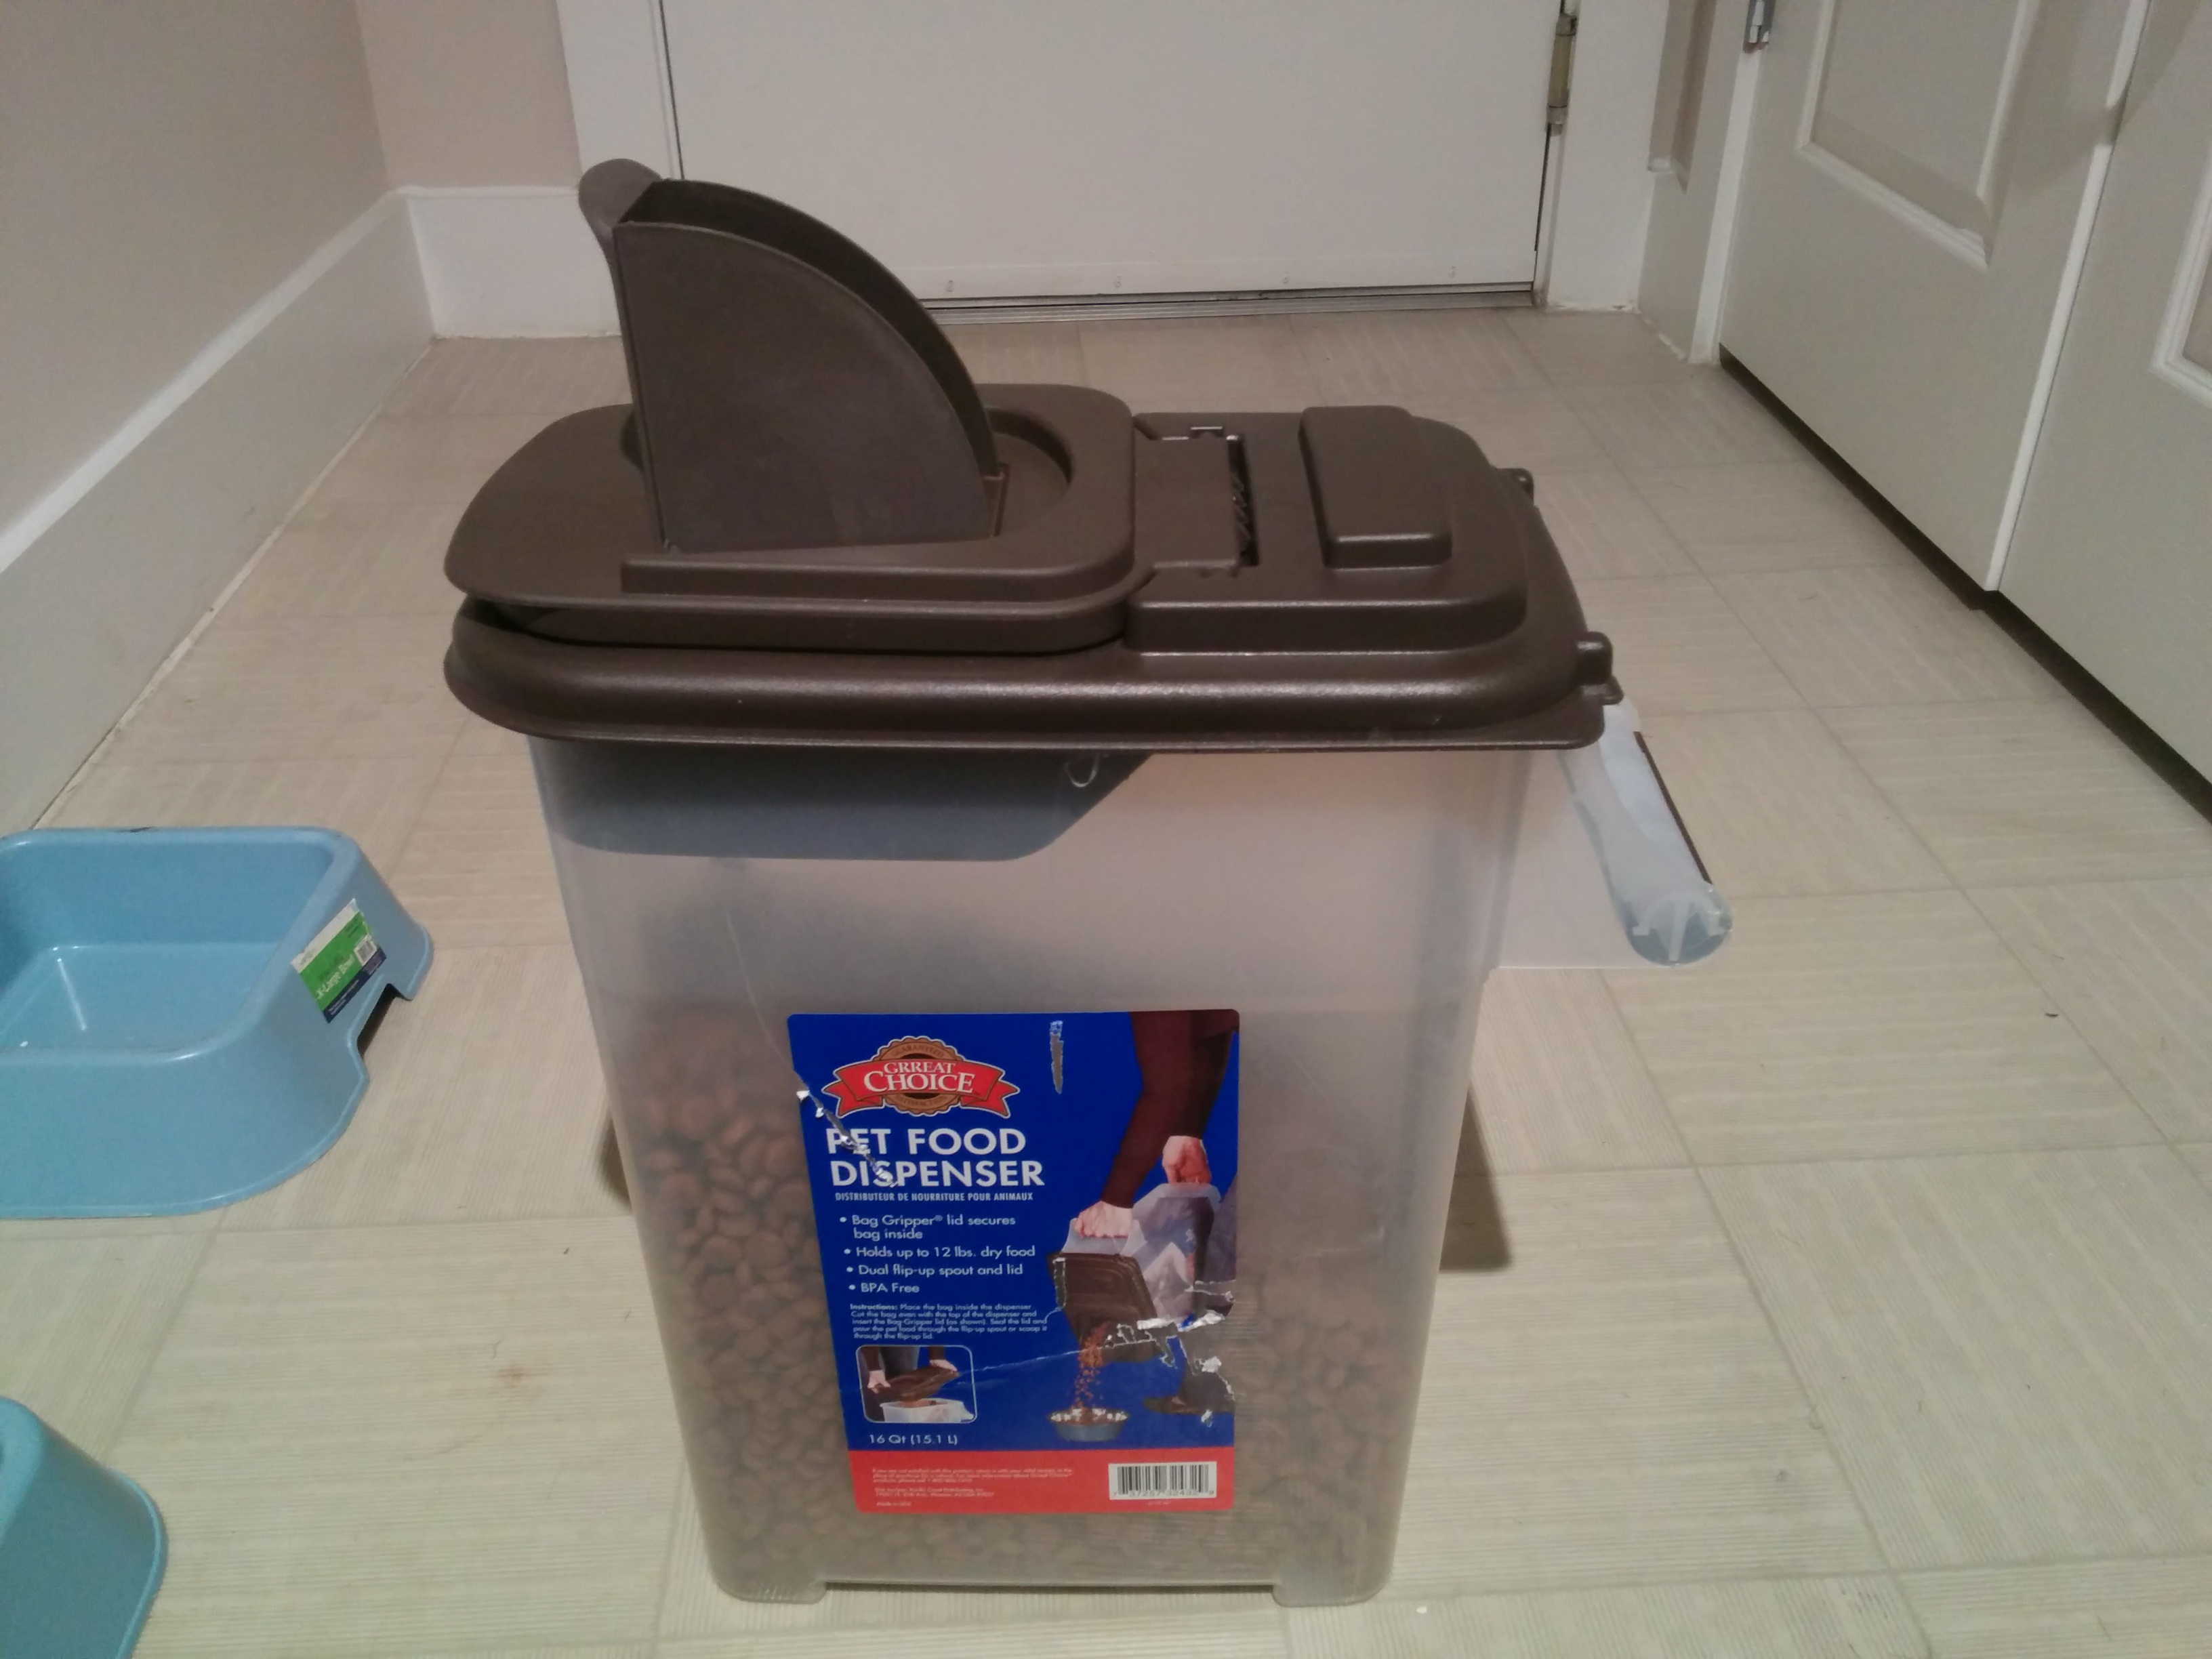
\includegraphics[width=.35\textwidth]{./images/how_to/feed_max/food_container_open.jpg}
    \caption*{The food container being opened correctly.}
    \label{fig:food_container_open}
\end{figure}

\bigskip

\begin{figure}[h!]
    \centering
    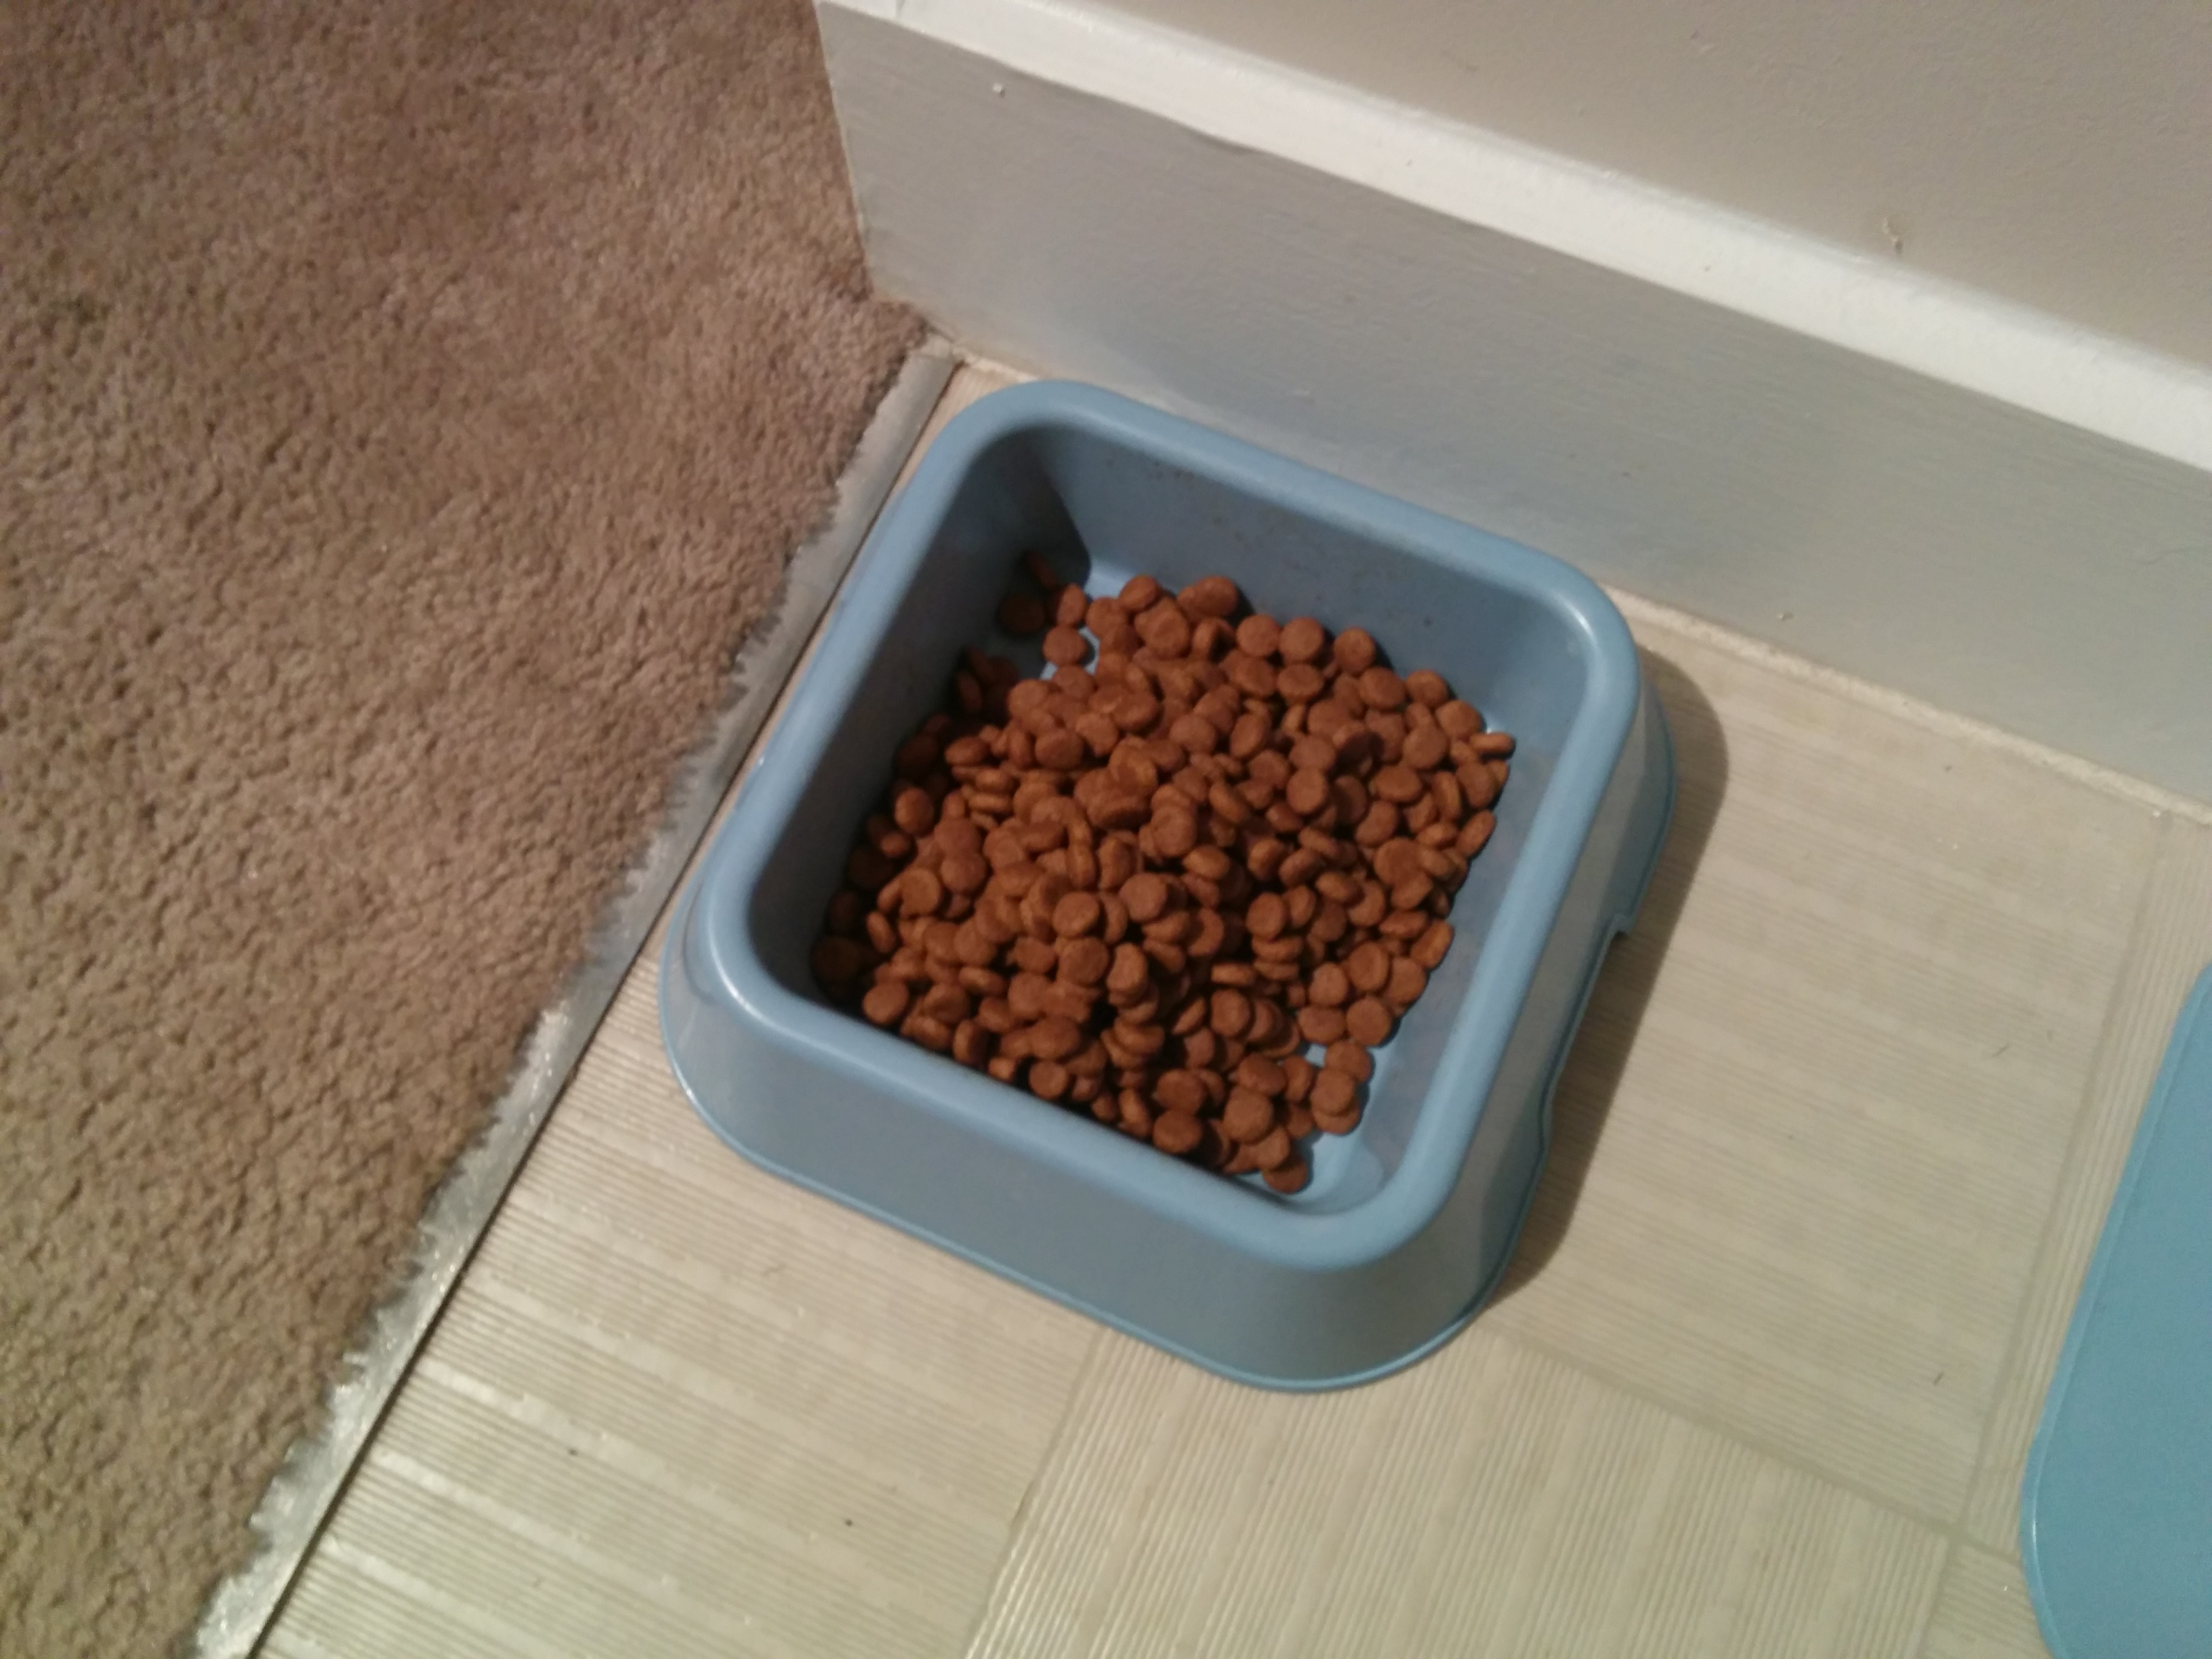
\includegraphics[width=.35\textwidth]{./images/how_to/feed_max/food_bowl_filled.jpg}
    \caption*{Max's food bowl filled to the proper amount.}
    \label{fig:food_bowl_filled}
\end{figure}

\subsection{How to walk Max}
\begin{enumerate}\label{itm:how_to_walk}
    \item Call Maxwell to the door saying, ``Let's go outside!''
    \item Get Maxwell to sit, waiting
    \item Go outside, while walking keep Max close by or in heel with his e-collar.
    \item If you're using the leash it should be loose at your side.
    \item Maxwell should always walk on your left side.
        Heel him or correct him if he's on the wrong side.
    \item Don't let him lollygag.
        Use heel strictly to get him in place while walking.
    \item You can release him to let him run off and explore, but
        be sure to call him back with the e-collar before returning to heel.
\end{enumerate}

\subsection{How to clean up an accident}
\begin{enumerate}\label{itm:how_to_clean_accident}
    \item Identify the spot where Max has gone
    \item Mark off the area, and put Max away
    \item Get the peepee solution, and paper towels from his bag
    \item Get a trashcan or other receptacle for the soaked paper towels
    \item Soak up the accident with the paper towels (Note: this will be disgusting)
    \item When the paper towels come away generally dry, open the peepee solution to ``spray''
    \item Spray the solution around the area so that it soaks into the carpet
    \item Let sit for 3-5 minutes
    \item Scrub the solution into the carpet with paper towels
    \item Soak up the excess solution with paper towels
    \item Repeat as necessary
\end{enumerate}

\clearpage
\section{Notes and Other Information}

Welcome to the end of the manual.
By this time you should be sufficiently prepared to watch Maxwell for a short period of time.
This final section contains some notes and other information that you might find useful when watching Max.
I hope that you have enjoyed reading this manual, and if you have any questions, comments, or concerns as well as suggestions, please let me know!
Good luck watching Max.
I hope everything goes well!

\bigskip

\begin{enumerate}\label{itm:other_information}
    \item Things Maxwell likes
        \begin{enumerate}
            \item Going to Washington Square Park
            \item Going for walks around The Village
            \item Scratching behind his ears
            \item Tummy rubs
            \item Treats, chew toys, destruction in general
            \item Attention, lots of attention
            \item Cuddling
        \end{enumerate}
    \item Things Maxwell dislikes
        \begin{enumerate}
            \item Nail clippers (do not clip his nails)
            \item Baths
            \item Being moved forcefully (dragging by the collar, pushing him, etc\ldots)
        \end{enumerate}
    \item Things to note
        \begin{enumerate}
            \item Maxwell sheds a lot, I try to brush him every week
            \item Max can make lots of funny faces, please get pictures!
            \item Maxwell's ears naturally flip over; it's hilarious.
            \item Maxwell can be left alone for a maximum of 8 hours without food, water, or walks
            \item Maxwell is friendly and can be around children and other dogs
            \item Maxwell is a goofball
        \end{enumerate}
\end{enumerate}

\bigskip

\begin{figure}[H]
    \centering
    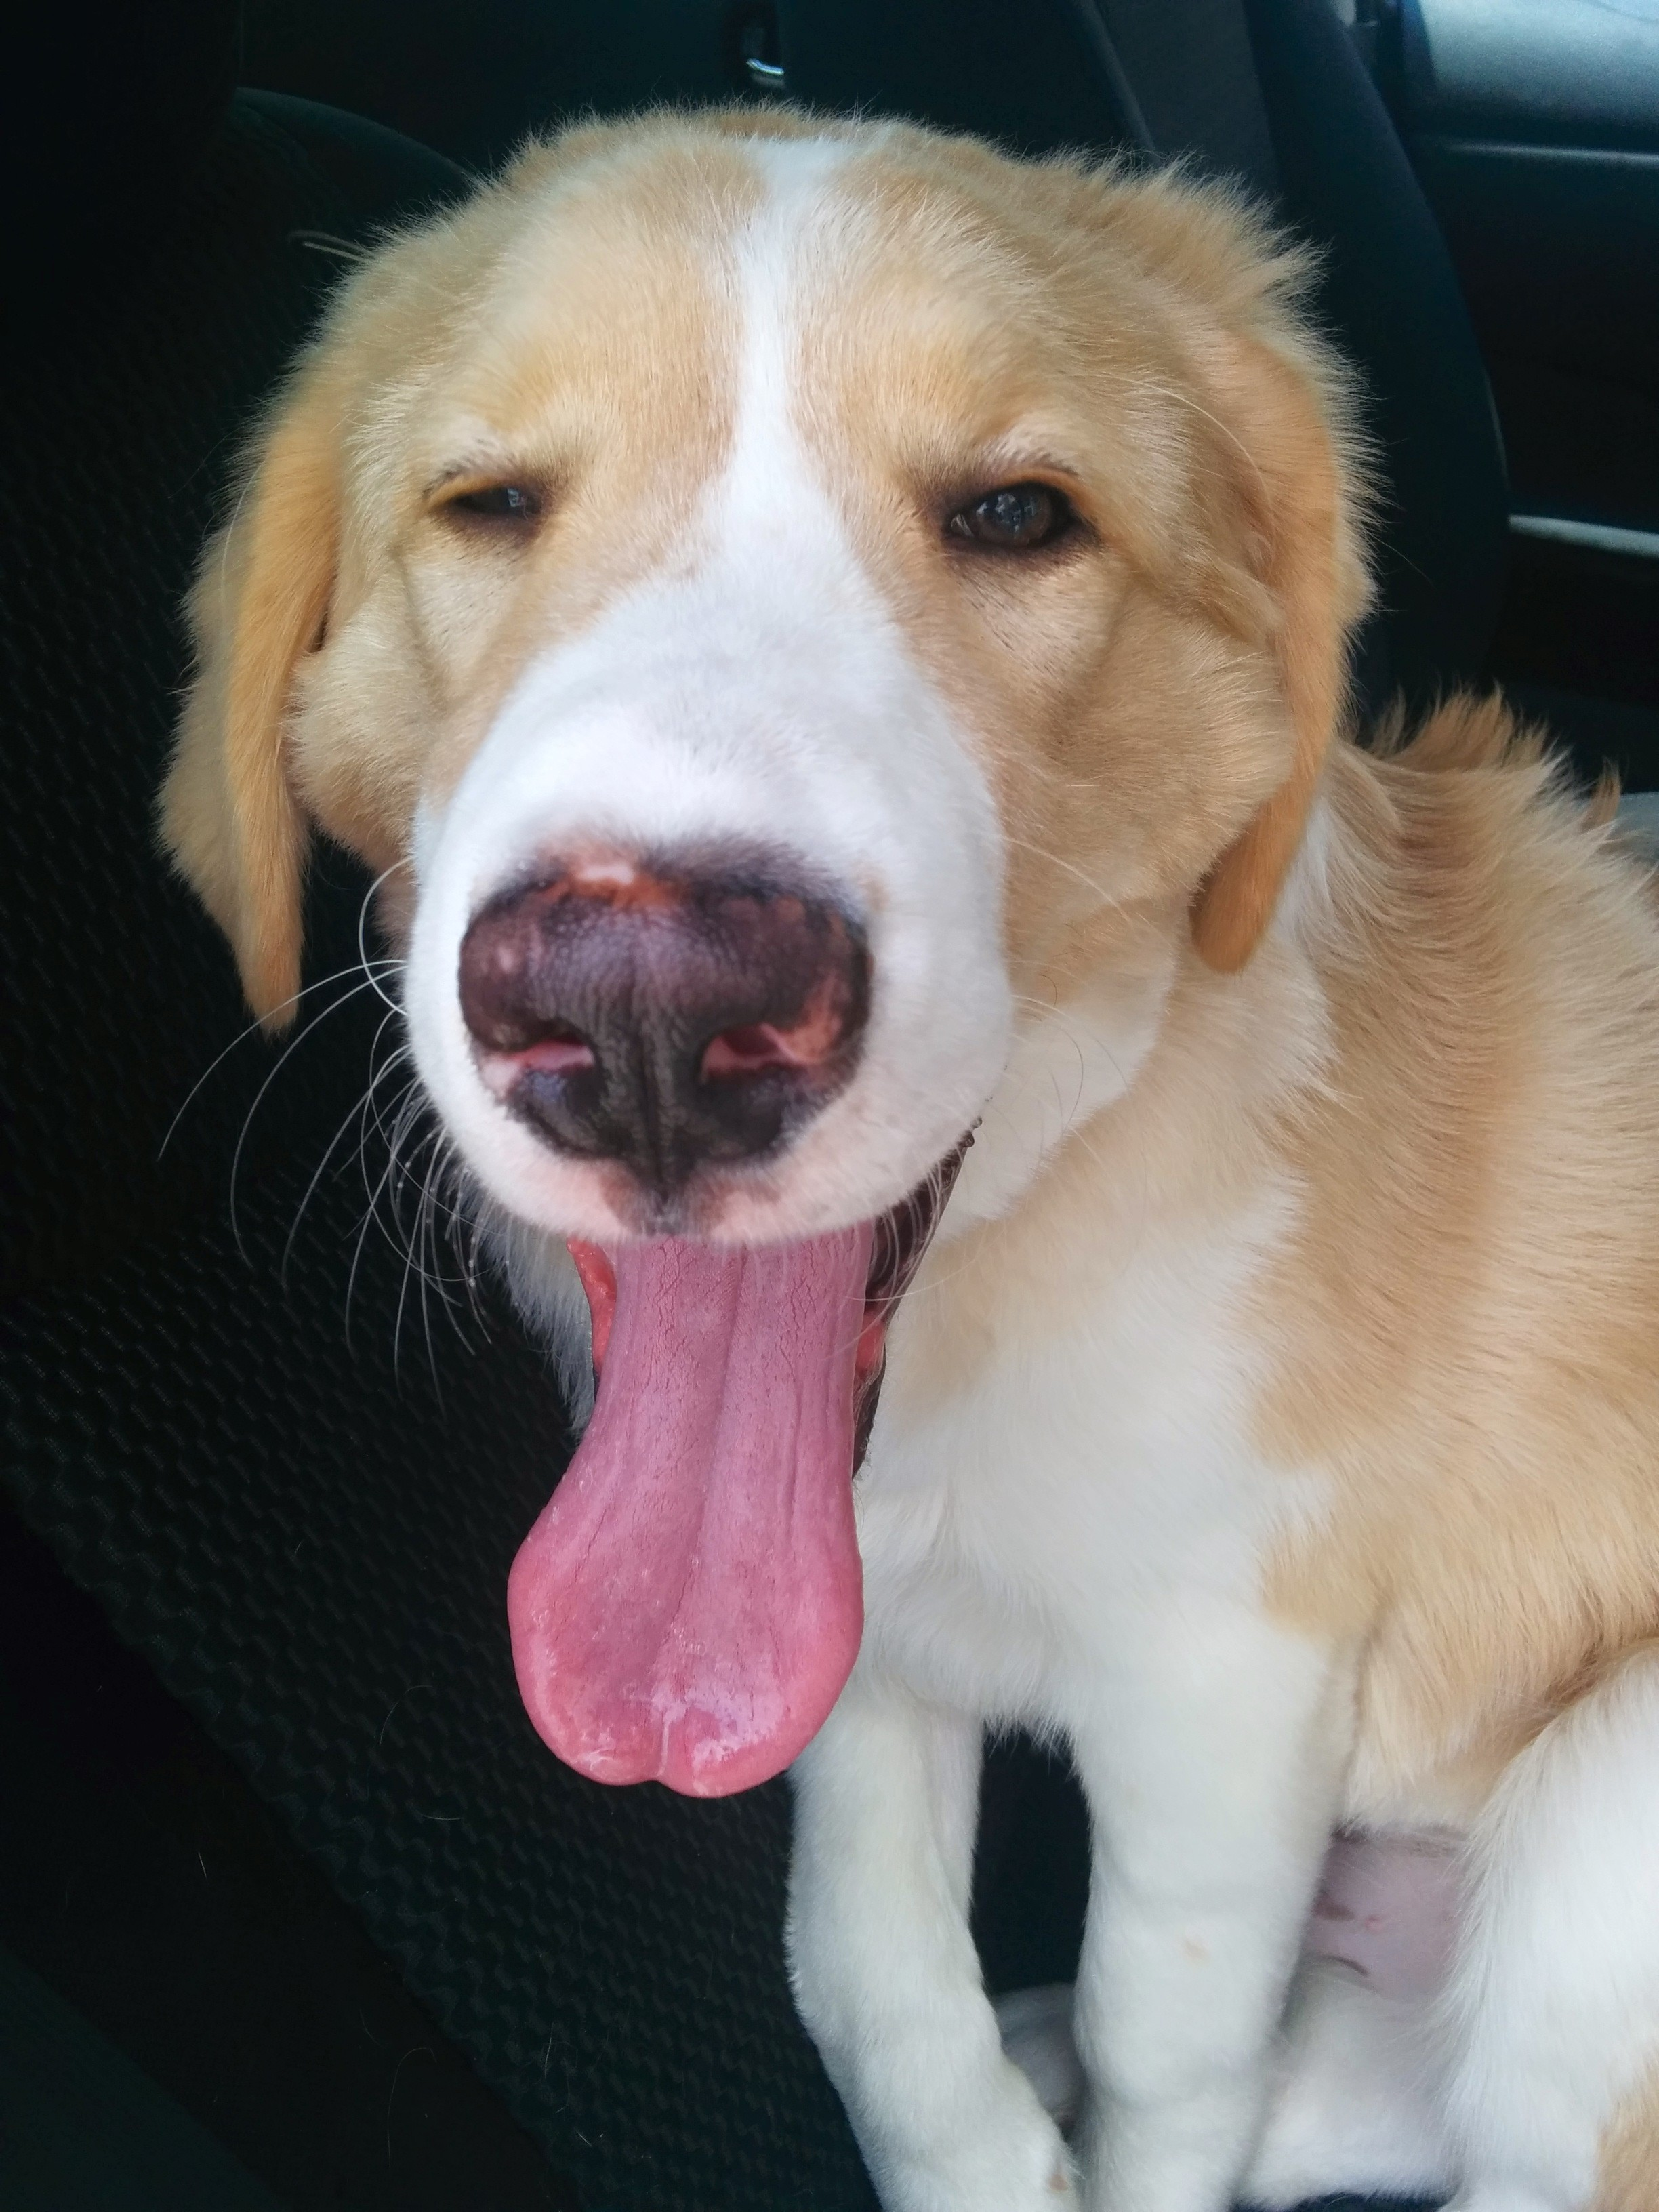
\includegraphics[width=.35\textwidth]{./images/max/totally_baked.jpg}
    \caption*{Maxwell looking totally baked.}
    \label{fig:totally_baked}
\end{figure}

\begin{figure}[H]
    \centering
    
\includegraphics[width=.35\textwidth]{./images/max/natural_ears.jpg}
    \caption*{Maxwell's ears in their natural position.}
    \label{fig:natural_ears}
\end{figure}

\begin{figure}[H]
    \centering
    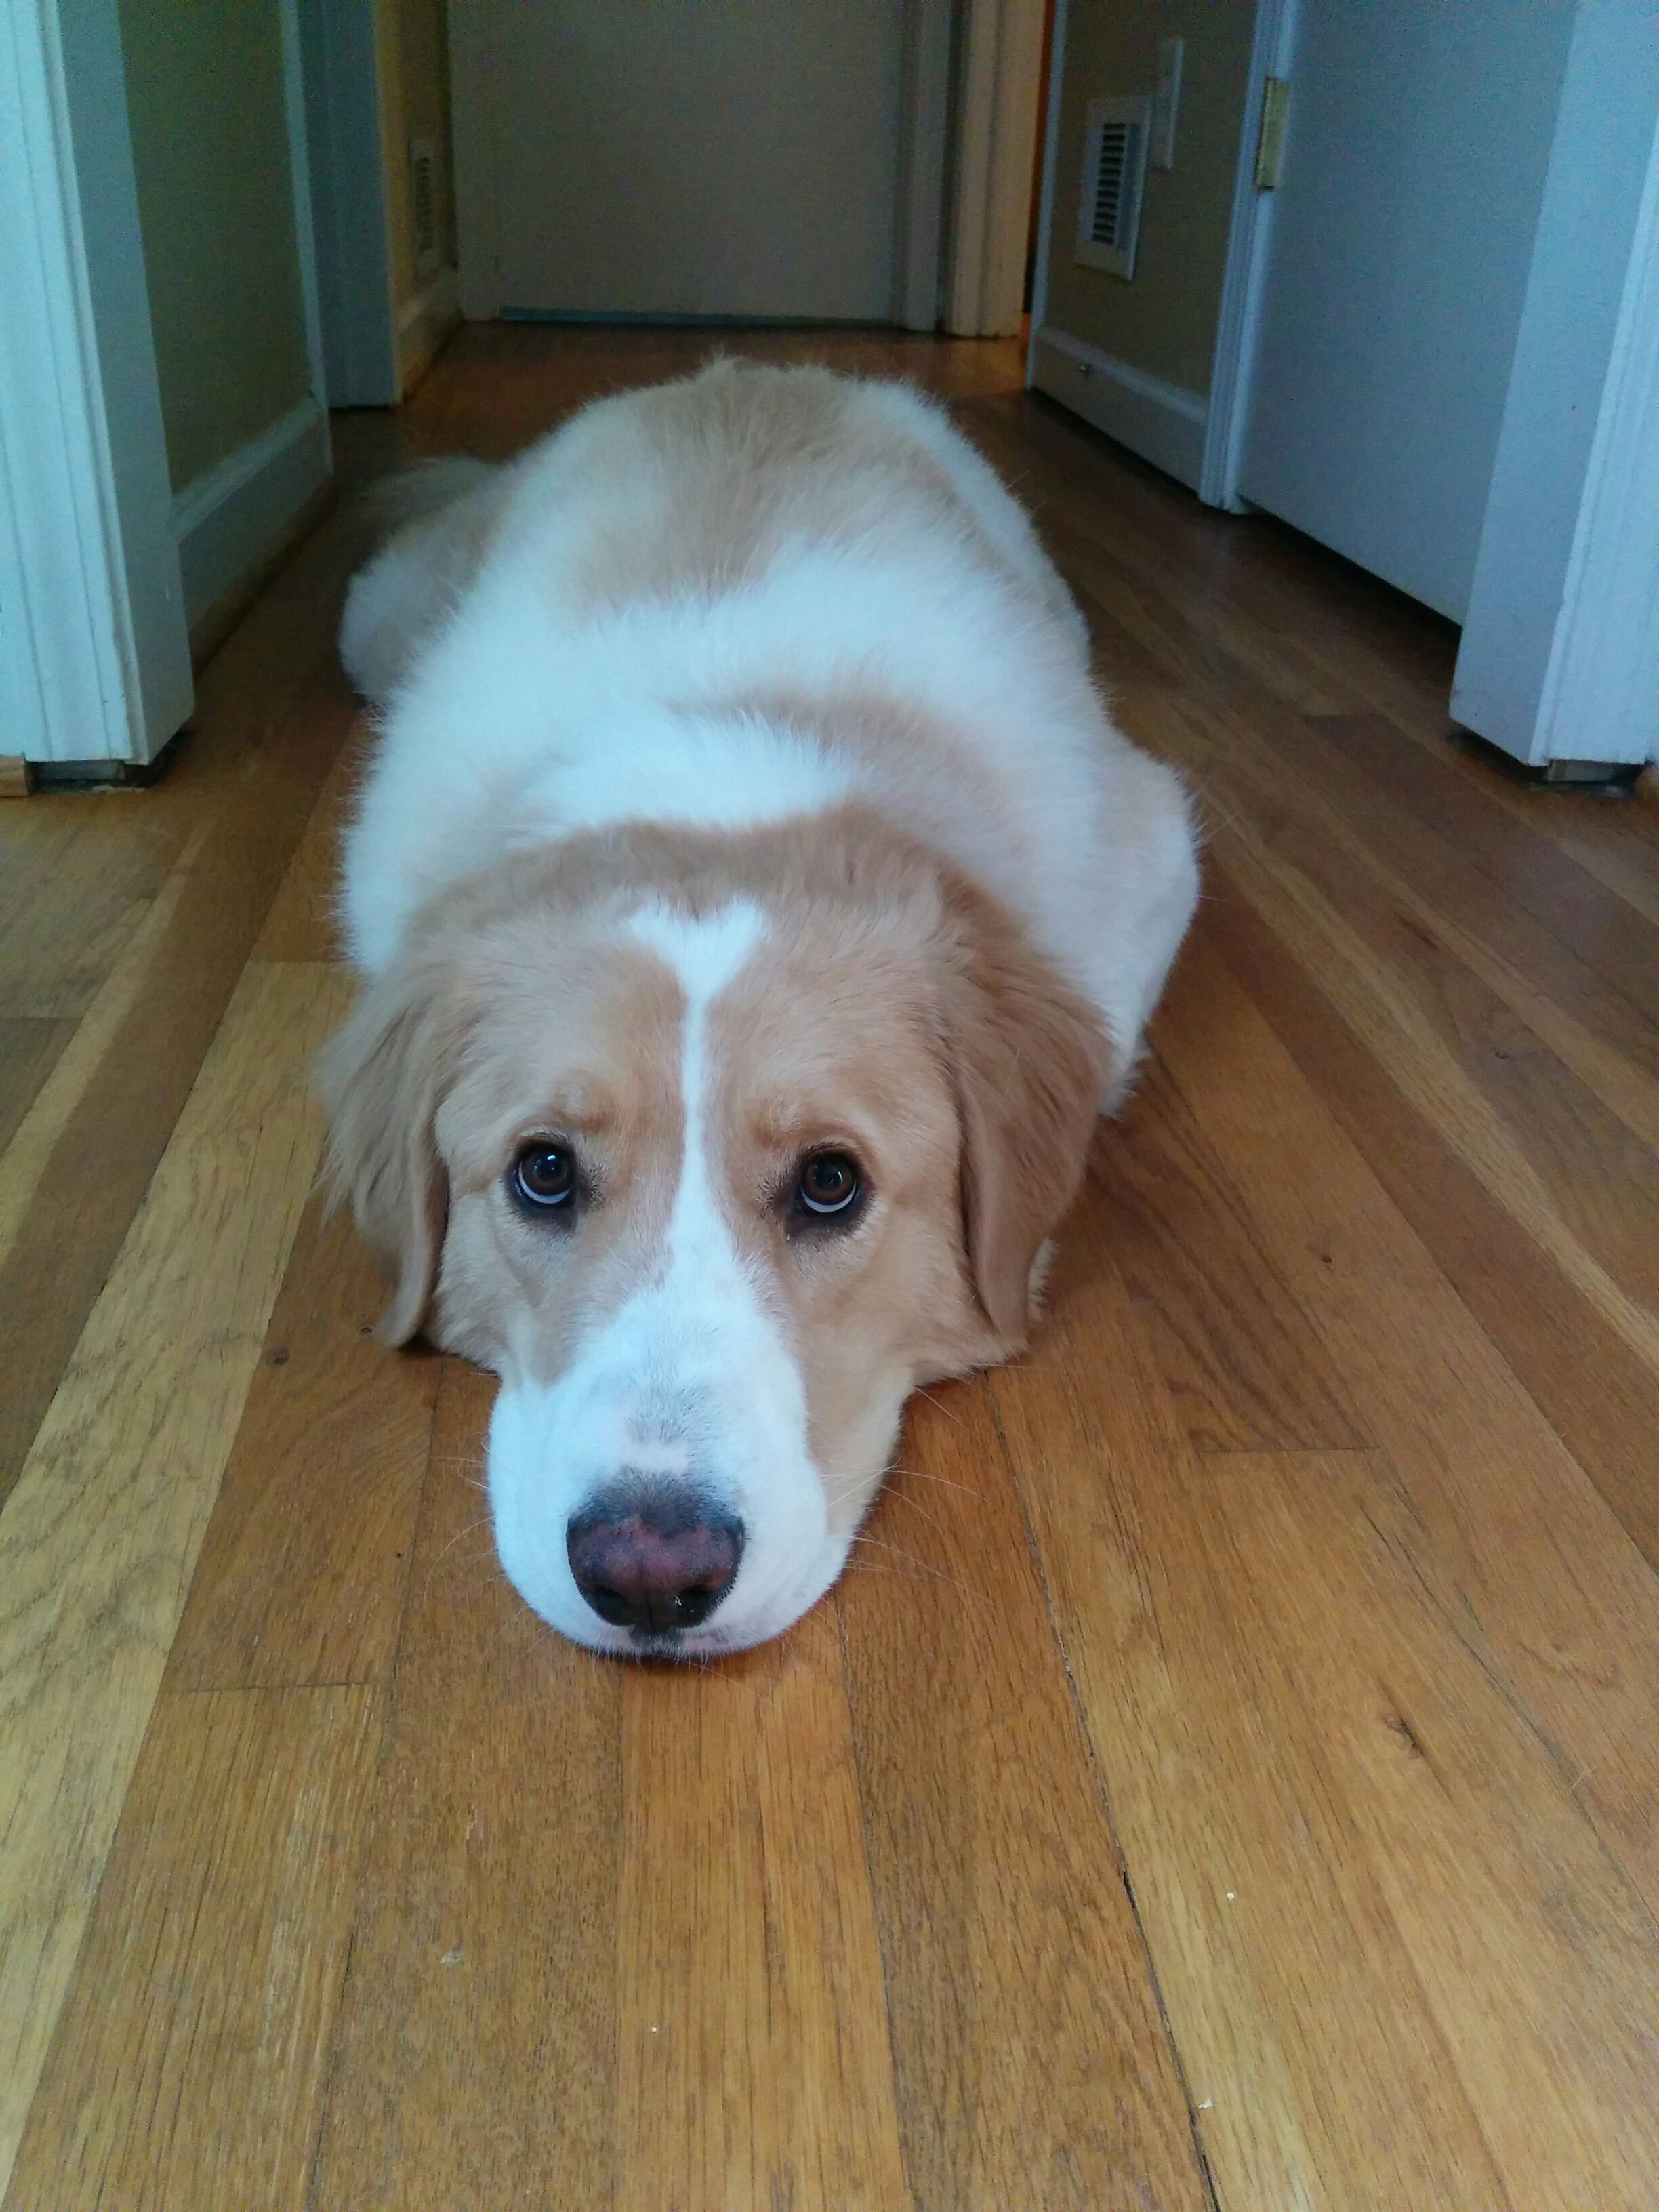
\includegraphics[width=.35\textwidth]{./images/max/rocket_ship.jpg}
    \caption*{``Look at that face''}
    \label{fig:rocket_ship}
\end{figure}

\end{document}
